\documentclass[conference]{IEEEtran}
\IEEEoverridecommandlockouts
% The preceding line is only needed to identify funding in the first footnote. If that is unneeded, please comment it out.
\usepackage[portuges,brazil,english]{babel}
\usepackage[utf8]{inputenc}
\usepackage{amsmath,amssymb,amsfonts}
\usepackage{algorithmic}
\usepackage{graphicx}
\usepackage{textcomp}
\usepackage{float}
\def\BibTeX{{\rm B\kern-.05em{\sc i\kern-.025em b}\kern-.08em
    T\kern-.1667em\lower.7ex\hbox{E}\kern-.125emX}}

\usepackage{subcaption}
\usepackage[style=mla,guessmedium=false,backend=bibtex]{biblatex}
\addbibresource{report.bib}

\begin{document}

\renewcommand{\figurename}{Fig.}
\renewcommand{\refname}{Referências}

\title{Regressão Logística e Redes Neurais para Classificação de Vestuário (Fashion MNIST)}

\author{\IEEEauthorblockN{Carolina F. Cuba}
\IEEEauthorblockA{
226004 \\
carolinacuba23@gmail.com}
\and
\IEEEauthorblockN{Leonardo de Melo Joao}
\IEEEauthorblockA{
228118 \\
l228118@g.unicamp.br}}

\maketitle

\section{Introdução}	

	O intuito desse projeto é estudar de maneira didática o funcionamento  de algoritmos classificadores, dentre eles: Regressão Logística para multiclasses e Redes Neurais Artificiais. Para tanto, apresentaremos duas versões simples de Redes Neurais e Regressões Logísticas. 
	
	As versões de cada algoritmo serão testados na base de dados \textit{Fashion MNIST}. O desafio proposto pela base é, dada uma imagem de vestuário classificá-la em 1 dentre 10 possíveis classes. No decorrer dos testes demonstraremos as dificuldades de seleção dos hiper-parâmetros desses algoritmos, bem como suas performances na base selecionada.
	
\section{Conjunto de Dados: Fashion MNIST}

	A\textit{ Fashion MNIST,} proposta por \citeauthor{xiao2017/online} (\citeyear{xiao2017/online}), é uma base criada especialmente para \textit{benchmarking} de algoritmos de \textit{machine learning}, como informado pelo próprio autor.
	
	O desafio é classificar as imagens que a compõe entre 10 possíveis classes de vestuário, sendo elas: [0] Camiseta ("T-shirt/top"); [1] Calça ("Trouser"); [2] Pullover; [3] Vestido ("Dress"); [4] Casaco ("Coat"); [5] Sandália ("Sandal"); [6] Camisa ("Shirt"); [7] Tênis ("Sneaker"); [8] Bolsa ("Bag"); [10] Bota ("Ankle boot").
	
	Cada imagem possui 28x28 \textit{pixels} e são em tons de cinza, ou seja, cada imagem possui um vetor inicial de características de tamanho $28*28*1 = 784$, onde 1 é o número de bandas de uma imagem em escala de cinza.
	
	A base é composta por 60.000 imagens para treinamento e 10.000 para teste. As imagens de teste só foram utilizadas depois do modelo final ser escolhido. Para escolher esse modelo, testes de validação foram realizados no conjunto de treinamento que, por sua vez, foi dividido com 70\% para treino e 30\% para validação.
	
\section{Regressão Logística}

Regressão logística é uma técnica estatística muito utilizada na área de Aprendizado de Máquina para resolver problemas de classificação. Ela utiliza a função de \textit{sigmoid} para mapear qualquer número real para um valor entre 0 e 1. Essa característica mostrou-se fundamental pois o método trabalha com probabilidades para predizer a melhor classe dado uma determinada amostra da base. \par

Inicialmente, a Regressão Logística foi criada para resolver problemas de classificação binária. No entanto, estudos foram propostos para adapta-la a casos em que mais classes estão envolvidas. Neste trabalho, implementamos e comparamos duas dessas principais adaptações: \textit{One-vs-All} e \textit{SoftMax}.

\subsection{One versus All}
O \textit{OnevsAll} é uma estratégia que propõe o treinamento de vários classificadores diferentes de forma que, em cada um deles, uma das classes seja tida como a positiva, e as demais consideradas uma única classe negativa.\par
Cada classificador produz um vetor de confiança onde ele salva a probabilidade de uma dada amostra pertencer a determinada classe. Sendo assim, no \textit{One-vs-All}, criamos uma matriz de confiança (classes x amostra) para retornar o classificador cujo valor de certeza é maior para classificação daquela determinada amostra.\par
Esta estratégia é muito utilizada (inclusive em outros classificadores famosos, como o SVM), mas possuí alguns problemas. Primeiramente, a escala dos valores de confiança pode acabar sendo diferente para cada classificador binário. Além disso, mesmo se a distribuição de amostras de treino for balanceada, cada classificador binário vê apenas distribuições não balanceadas visto que o conjunto de amostras negativas sempre será muito mais alto do que o de amostras positivas.

\subsection{Softmax}

O \textit{Softmax}, por sua vez, é uma generalização da Regressão Logística e, como o próprio nome sugere, envolve substituir a função \textit{sigmoid}, que é o núcleo da Regressão Logística tradicional, pela função \textit{softmax} definida a seguir:

\begin{equation*}
 \textit{softmax}(z)^i = \frac{e^{z^i}}{\sum\limits_{j=0}^k e^{z_k^i}  }
\end{equation*}

A equação de z já é bem conhecida dos estudos de Regressão Logística, e Linear, e consiste em multiplicar uma matriz de pesos \textbf{w} por uma matriz de \textit{features} \textbf{x}. A esse resultado se deve somar um vetor escalar \textbf{b} cujo tamanho deve ser igual ao número de classes do problema. O resultado z é aplicado à função \textit{Cross-Entropy} para calcular o valor de erro gerado pelo modelo da iteração atual.\par
 Assim como os rótulos de \textit{Ground Truth}, aqueles que foram preditos devem estar no formato \textit{One Hot Encoding} que é umas das estratégias fundamentais para conseguirmos encontrar o resultado de um problema de multi classificação sem utilizar vários classificadores.




\section{Redes Neurais Artificiais}

	Como um exemplo de computação bio inspirada, as Redes Neurais Artificiais são uma abstração computacional para representação de um modelo cerebral. Para tanto, neurônios foram modelados como perceptrons.E seu funcionamento é igual ao de uma regressão logística: um conjunto de dados ponderados por um vetor de pesos entram em um perceptron; esses dados são combinados e submetidos à uma função de ativação; quando o valor de saída da função de ativação é maior que um limiar escolhido, é dito que o perceptron ativou. Uma representação visual de um perceptron pode ser vista na Figura 1.
	
  
  \begin{figure}[!h]
      \centering
      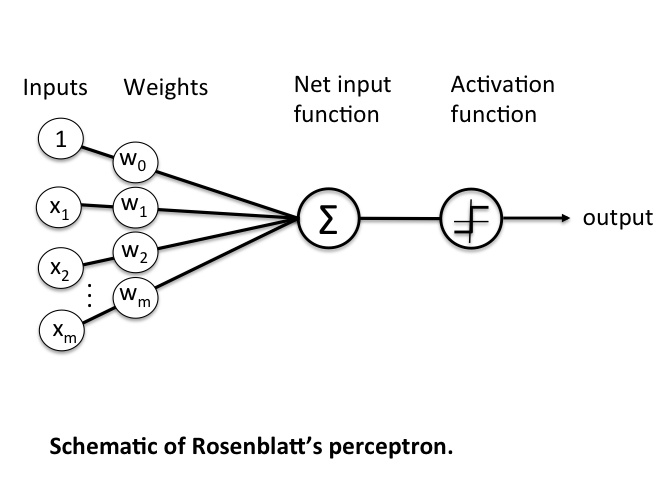
\includegraphics[width=0.6\columnwidth]{images/perceptron.png}
      \caption{Perceptron de Rosenblatt}
      \label{fig1}
\end{figure}  
  
  Em linhas gerais, uma Rede Neural é um conjunto de perceptrons interconectados onde a saída de um conjunto de perceptrons é ponderada por um vetor de pesos e dada como entrada de outro conjunto de perceptrons. 
  
  A camada de entrada (\textit{Input Layer}) envia os dados de entrada ponderados pelos seus respectivos pesos para a camada escondida (\textit{Hidden Layer}). Em seguida, cada neurônio da camada escondida combina seus valores de entrada e os submete a uma função de ativação. O resultado das ativações é ponderado por outro vetor de pesos e enviado ou a uma camada de saída (\textit{Output Layer}) ou a outra camada escondida que repete o mesmo processo da camada anterior. A ativação da camada de saída é o que define a classe na qual o objeto de entrada pertence. 
  
  A quantidade de camadas escondidas e de neurônios em cada camada pode variar dependendo da complexidade do problema. Nesse trabalho, esses hiperparâmetros foram definidos de maneira empírica, bem como o valor da constante de aprendizagem \textit{learning rate}). Os testes referêntes à escolha desses parâmetros podem ser vistos nas tabelas: Tabela 1 e Tabela 2
  
  Assim como na regressão logística, uma Rede Neural classifica problemas binários e para resolver problemas multiclasse, utiliza-se a função \textit{softmax} como função de ativação da camada de saída.
  
  Contudo, as MLPs só puderam ser utilizadas devido a uma técnica de aprendizagem baseado no erro retropropagado pelas camadas, proposta por \citeauthor{rumelhart1986learning} (\citeyear{rumelhart1986learning}), \textit{backpropagation}. Consiste em calcular derivadas subsequentes usando a regra da cadeia, propagando o erro para as camadas mais distantes, identificando a relevância de cada peso no erro final.
  
  
% \section{Funções de ativação}
% 	Antes dos testes serem apresentados, faz-se necessário uma breve descrição das 3 funções de ativação implementadas: [1] sigmoid; [2] tangente hiperbólica; [3] rectified linear unit (ReLU).
	 
% \subsection{Sigmoid}

% 	A sigmoid é primeira função a ser implementada em um perceptron, vindo de herânça da regressão logística. Ela é uma função descrita pela equação: 

% \begin{equation}
% sigmoid(x) = \dfrac{1}{1 + e^{-x}}
% \end{equation}	

% 	O problema dessa função é que os valores de saída estão entre 0 e 1. Isso causa problemas no calculo da descida de gradiente uma vez que devido aos valores de saída serem sempre baixos, os valores dos pesos variam muito pouco nas suas atualizações. Esse problema é chamado de \textit{vanishing gradient} e pode ser vistos nesse trabalho nos testes das redes com duas camadas.
	
% 	Para a atualização de parâmetros, a derivada dessas funções de ativação devem ser utilizadas. A derivada da sigmoid é descrita pela equação:
	

% \begin{equation}
% \dfrac{d}{dx}sigmoid(x) = \dfrac{1}{1 + e^{-z}} * (1 - \dfrac{1}{1 + e^{-z}})
% \end{equation}	

% \subsection{Tangente Hiperbólica}
  
% 	A tangente hiperbólica (representada geralmente como tanh), é similar à sigmoid, mas seus valores variam entre -1 e 1. Entretanto, ela ainda apresenta o problema do \textit{vanishing gradient}. A tanh é definida pela equação:
  
% \begin{equation}
% tanh(x) = \dfrac{2}{1+e^{-2x}} - 1
% \end{equation}

% 	Sua derivada, utilizada no backpropagation, é definida por:
% \begin{equation}
% \dfrac{d}{dx}tanh(x) =  1 - (\dfrac{2}{1+e^{-2x}} - 1)^2
% \end{equation}	

% \subsection{Rectified Linear Unit (ReLU)}

% 	Para resolver o problema do vanishing gradient, \citeauthor{nair2010rectified} (\citeyear{nair2010rectified}) propôs a ReLU. Essa função é definida como 0 quando $x	\leq 0$ e $x$ quando $x>0$. Isso faz com que os valores tenham um peso maior no algoritmo do gradiente descendente. Sua representação matemática é:
	
% \begin{equation}
% ReLU(x) =  max(0,x)
% \end{equation}

% 	Sua derivada, utilizada na backpropagation, é 1 quando $x>0$ e 0 quando $x \leq 0$.
	
\section{Criando e escolhendo os modelos}

Nesta seção apresentaremos os testes realizados para cada um dos modelos criados.A análise do comportamento de cada modelo foi feita utilizando os custos finais de convergência ao variar os valores de \textit{learning rate} e o número de iterações. Além disso, após descobrir os melhores parâmetros, criamos uma tabela para mostrar as métricas de performance: Precisão, \textit{Recall}, \textit{F1-Score}. Também foram medidos o tempo de computação, em segundos, fazendo uma média de três execuções consecutivas para um mesmo modelo.

\subsection{Regressão Logística: One versus All e Softmax}

Quanto a Regressão Logística com \textit{softmax} podemos perceber que o crescimento do tempo de processamento foi diretamente proporcional à quantidade de iterações definidas%.Quanto ao \textit{learning rate}, se consideramos o mesmo número de iterações, os valores de tempo foram maiores para valores baixos de \textit{learning rate} (LR), por alguma razão, no entanto, isso não ocorreu para 2000 iterações
. Além disso, para um LR igual a  0.3, a convergência do custo foi irregular, ou seja, com valores altos e baixos, mostrando que esse valor é muito alto e o algorítmo da descida do gradiente teve problemas na convergência. Esse problema não ocorreu nos outros dois valores. Pudemos perceber também que LR igual 0.1 convergiu para um valor menor de custo, e mais depressa. Portanto, selecionamos esse valor de \textit{learning rate} para fazer testes de performance. \par
Analisando a tabela referente à Regressão Logística com \textit{One-vs-All}, observamos que, assim como na anterior, o número de iterações influencia diretamente no tempo gasto do treinamento.Diferente do \textit{softmax}, este método apresentou resultados melhores para o LR igual a 0.3, no entanto demorou muito mais tempo em comparação com o \textit{softmax}.

\begin{table}[ht!]
 \begin{center}
  \caption{Performance tests for different learning rates and number of iterations (\textbf{One-vs-All})}
  \label{table:table1}
  \begin{tabular}{ |c|c|c|c|c| }
   \hline
    Iterations & Learning Rate & Convergency Cost & Time(s)\\
   \hline
   500 & 0.3 & 0.9877 & 186.28 \\ 
                     & 0.1 & 1.88 & 184.70 \\
                     & 0.005 & 2.07 & 211.55 \\
   \hline
   1000 & 0.3 & 0.9674 &376.26 \\ 
                     & 0.1 & 0.9676 & 373.90 \\
                     & 0.005 & 1.113 & 370.07 \\
   \hline
   2000 & 0.3 & 0.8859 & 707.84 \\ 
                     & 0.1 & 1.4669 & 776.09 \\
                     & 0.005 & 1.0016 & 839.91 \\


 \hline
 \end{tabular}
 \end{center}
\end{table}



\begin{table}[ht!]
 \begin{center}
  \caption{Performance tests for different learning rates and number of iterations (\textbf{Softmax})}
  \label{table:table1}
  \begin{tabular}{ |c|c|c|c|c| }
   \hline
    Iterations & Learning Rate & Convergency Cost & Time(s)\\
   \hline
   500 & 0.3 & 4262.28 & 82.37 \\ 
                     & 0.1 & 4005.46 & 88.20 \\
                     & 0.005 & 4434.78 & 92.12 \\
   \hline
   1000 & 0.3 & 3950.47 & 173.36\\ 
                     & 0.1 & 3655.32 & 179.77 \\
                     & 0.005 & 3977.04 & 180.65 \\
   \hline
   2000 & 0.3 & 3691.28 & 306.51 \\ 
                     & 0.1 & 3397.58 & 308.11 \\
                     & 0.005 & 3644.95 & 289.90 \\


 \hline
 \end{tabular}
 \end{center}
\end{table}

	Com esses resultados, o melhor modelo de Regressão Logística com \textit{softmax} foi gerado a partir de 2000 iterações e \textit{learning rate} igual a 0.1. Para a versão com One-vs-All, utilizamos os valores de 2000 iterações e LR igual a 0.3. Comparando as duas tabelas, foi possível concluir que o método de One-Vs-All é um pouco melhor do que o por \textit{softmax}, no entanto, este é muito mais rápido.

\begin{table}[h!]
 \begin{center}
  \caption{Precision, Recall e F1-Scores do Conjunto de Validação (\textbf{Softmax})}
  \label{table:table3}
  \begin{tabular}{ |c|c|c|c| }
   \hline
   Classe & Precision & Recall & F1-Score\\
   \hline
   0 & 0.82 & 0.77 & 0.8 \\
   1 & 0.95 & 0.97 & 0.96 \\
   2 & 0.73 & 0.74 & 0.74 \\
   3 & 0.87 & 0.83 & 0.85 \\
   4 & 0.77 & 0.72 & 0.74 \\
   5 & 0.87 & 0.95 & 0.91 \\
   6 & 0.56 & 0.65 & 0.6 \\
   7 & 0.92 & 0.9 & 0.91 \\
   8 & 0.93 & 0.94 & 0.94 \\
   9 & 0.94 & 0.89 & 0.92 \\
   \hline
 \end{tabular}
 \end{center}
\end{table}

\begin{table}[h!]
 \begin{center}
  \caption{Precision, Recall e F1-Scores do Conjunto de Validação (\textbf{One-vs-All})}
  \label{table:table3}
  \begin{tabular}{ |c|c|c|c| }
   \hline
   Classe & Precision & Recall & F1-Score\\
   \hline
   0 & 0.87 & 0.76 & 0.81 \\
   1 & 0.95 & 0.97 & 0.96 \\
   2 & 0.84 & 0.65 & 0.73 \\
   3 & 0.87 & 0.82 & 0.85 \\
   4 & 0.74 & 0.74 & 0.74 \\
   5 & 0.91 & 0.94 & 0.93 \\
   6 & 0.4 & 0.78 & 0.53 \\
   7 & 0.92 & 0.9 & 0.91 \\
   8 & 0.95 & 0.92 & 0.94 \\
   9 & 0.95 & 0.93 & 0.94 \\
   \hline
 \end{tabular}
 \end{center}
\end{table}

	\bigskip
	\bigskip
	\bigskip
	
	Contudo, quando comparado com os resultados das Redes Neurais, os modelos gerados pelas regressões logísticas não foram melhores e, portanto, não foram escolhidos como modelos finais.




\subsection{Rede Neural}

	Começamos implementando uma Rede Neural com apenas 1 camada escondida. Todos os testes foram feitos com 3000 épocas, valor utilizado para manter um tempo de execução aceitável. Os valores da constante de aprendizagem, do número de neurônios e a função de ativação utilizada foram atribuídos empiricamente e seus respectivos testes estão descritos nas subções seguintes.
	
	As métricas de comparação dos modelos foram: precision, que mede quantas das amostras preditas como da classe $x$ realmente eram daquela classe; recall, que mede quantas das amostras da classe $x$ foram corretamente preditas como $x$; e o f1-score é uma combinação das outras duas métricas.
	
	As funções sigmoid e tanh estavam funcionando corretamente e convergindo para um erro mínimo nos primeiros testes. Entretanto quando a relu era aplicada os valores dos pesos começavam a tender para infinito positivo e negativo.
	
	Após alguns testes e pesquisas, descobrimos que quando utiliza-se relu o valor inicial dos pesos não podem ser muito elevados, uma vez que esse valor não é normalizado entre $(0,1)$ ou entre $(-1,1)$ como é o caso na sigmoid e na tanh.
	
	Nesse cenário, os valores dos pesos foram inicializados com valores menores que $1*10^{-2}$. Com essa alteração, todas funções de ativação começaram a convergir para o mínimo e os testes puderam ser feitos. Contudo, nos testes com as redes com duas camadas e mais neurônios, a função sigmoid não convergia com pesos inicialmente baixos, devido ao problema do \textit{Vanishing Gradient}, mas a tanh não apresentou problemas. Isso pode ser observado na Tabela 3.
	
	Concluímos por esses testes que as funções de ativação são muito sensíveis aos valores dos pesos iniciais. Por consequência, as redes neurais são muito sensíveis à escolha dos hiperparâmetros

\subsubsection{Uma camada oculta}
	
	A Tabela 1 mostra alguns dos testes executados. Antes desses testes o \textit{learning rate} já tinha sido testados com valores menores e mostrava necessitar muitas iterações para convergir para valores próximos. Note que NHL na tabela é o número de neurônios na camada escondida.
	
\begin{table}[h!]
 \begin{center}
  \caption{Testes de Performance para NN com 1 Camada Oculta}
  \label{table:table1}
  \begin{tabular}{ |c|c|c|c|c|c|c| }
   \hline
   Ativação & LR & NHL & Precision & Recall & F1-Score & Tempo(s)\\
   \hline
   ReLU & 0.3 & 16 & 0.86 & 0.87 & 0.86 & 142.2 \\ 
                   & 0.1 & 16 & 0.85 & 0.86 & 0.85 & 166.1 \\
                   & 0.4 & 16 & 0.86 & 0.86 & 0.86 & 170.4 \\
                   & 0.3 & 32 & 0.87 & 0.88 & 0.87 & 233.4 \\
                   & 0.4 & 32 & 0.87 & 0.88 & 0.87 & 234.5 \\
   \hline
   Sigmoid & 0.3 & 16 & 0.85 & 0.85 & 0.85 & 165.6 \\ 
                     & 0.1 & 16 & 0.82 & 0.82 & 0.82 & 200.5 \\
                     & 0.4 & 16 & 0.86 & 0.86 & 0.86 & 196.1 \\
                     & 0.3 & 32 & 0.86 & 0.86 & 0.86 & 294.0 \\
                     & 0.4 & 32 & 0.86 & 0.87 & 0.86 & 293.9 \\	
   \hline
   Tanh & 0.3 & 16 & 0.86 & 0.87 & 0.86 & 159.9 \\ 
                     & 0.1 & 16 & 0.86 & 0.86 & 0.86 & 192.0 \\
                     & 0.4 & 16 & 0.86 & 0.86 & 0.86 & 194.3 \\
                     & 0.3 & 32 & 0.88 & 0.87 & 0.87 & 270.1 \\
                     & 0.4 & 32 & 0.87 & 0.87 & 0.87 & 284.2 \\

 \hline
 \end{tabular}
 \end{center}
\end{table}

	Nos testes feitos, o modelo que obteve os melhores resultados foi o que utilizava Relu, learning rate de 0.3 e 32 neurônios na camada escondida. Além disso, a ReLU obteve os melhores resultados em tempo, com a sigmoid sendo a mais lenta e com piores resultados.
	
	A tanh teve resultados bem próximos aos da ReLU mas levou mais tempo para executar.

\subsubsection{Duas camadas ocultas}

	Na rede com duas camadas ocultas com 16 neurônios em cada camada e learning rate 0.3, o valor dos custos a cada época não convergia sempre para o mínimo, saltando entre erros mais altos e mais baixos. Por conta disso, resolvemos experimentar com learning rates mais baixos.
	
	
\begin{table}[h!]
 \begin{center}
  \caption{Testes de Performance para NN com 2 Camadas Ocultas}
  \label{table:table6}
  \resizebox{\columnwidth}{!}{
  \begin{tabular}{ |c|c|c|c|c|c|c|c| }
   \hline
   Ativação & LR & NHL1 & NHL2 & Precision & Recall & F1-Score & Tempo(s)\\
   \hline
   ReLU & 0.1 & 16 & 16 & 0.84 & 0.84 & 0.84 & 194.1 \\
        & 0.3 & 16 & 16 & 0.84 & 0.85 & 0.84 & 199.1 \\
        & 0.1 & 32 & 16 & 0.85 & 0.85 & 0.84 & 256.0 \\
        & 0.3 & 32 & 16 & 0.86 & 0.87 & 0.86 & 274.5 \\
        & 0.1 & 16 & 32 & 0.84 & 0.84 & 0.84 & 220.6 \\
        & 0.3 & 16 & 32 & 0.86 & 0.86 & 0.86 & 319.9 \\
        & 0.1 & 32 & 32 & 0.87 & 0.87 & 0.87 & 287.2 \\
        & 0.3 & 32 & 32 & 0.86 & 0.86 & 0.86 & 319.5 \\
   \hline
   Softmax & 0.3 & 32 & 32 & 0.85 & 0.85 & 0.85 & 424.35 \\
   Softmax & 0.3 & 32 & 32 & 0.85 & 0.85 & 0.85 & 194.1 \\

 \hline
 \end{tabular}
 }
 \end{center}
\end{table}

\begin{table}[h!]
 \begin{center}
  \caption{Sigmoid com Diferentes Inicializações de Pesos}
  \label{table:table7}
  \begin{tabular}{ |c|c|c|c|c|c|c|c| }
   \hline
   LR & NHL1 & NHL2 & Precision & Recall & F1-Score & Pesos\\
   \hline
   0.3 & 32 & 32 & 0.85 & 0.85 & 0.85 & Altos \\
   0.3 & 32 & 32 & 0.77 & 0.76 & 0.76 & Baixos \\
   \hline
 \end{tabular}
 \end{center}
\end{table}
		
	
	Com os learning rates menores, o valor dos custos desceu continuamente. Porém, 3000 iterações não pareceu ser o suficiente para que a rede convergisse o necessário. Dito isso, o melhor modelo provavelmente seria outro caso o tempo de execução não tivesse sido pré-determinado. Infelizmente devido à data de submissão não pudemos realizar todos testes necessários.
	

	O problema descrito acima ocorreu em todos testes na rede com duas camadas. Acreditamos que por conta disso as redes com uma camada escondida acabaram tendo resultados mais satisfatórios.
	
	Como nos testes com uma camada oculta a ReLU foi a que mais se destacou, focamos em tentar encontrar um melhor modelo para ela. Essa é a razão para os testes terem sido majoritariamente focados nessa função de ativação.


	Nesses testes, o modelo que obteve os melhores resultados foi o que utilizava ReLU, com learning rate de 0.1 e com 32 neurônios em cada camada escondida. Entretanto, devido às limitações de tempo, como já discutido acima, o melhor modelo foi o encontrado com uma camada oculta.
	
\newpage
\section{Testando o modelo final no Dataset de Teste}

	O modelo final escolhido foi o criado a partir de uma rede com 1 hidden layer com 32 neurônio, 0.3 de learning rate e utilizando ReLU como função de ativação.	Para testar o modelo escolhido no conjunto de teste, nós retreinamos a rede com os mesmos hiperparâmetros mas utilizando todo o conjunto de trainamento. 
	
	O resultado final foi bem satisfatório em relação ao da validação, com $0.88$ de precision, $0.88$ de recall e $0.88$ de f1-score. Isso prova que o modelo não foi super treinado (overfitted). Para identificar quais classes tiveram mais problemas de classificação, geramos uma matriz de confusão e todas as métricas para cada classe individual:
	
	
	
\[
\begin{bmatrix}
    820 & 2   & 9   & 25  & 0   & 2   & 133 & 0   & 9   & 0 \\
    1   & 974 & 1   & 18  & 0   & 2   & 4   & 0   & 0   & 0 \\
    13  & 0   & 807 & 14  & 68  & 1   & 95  & 0   & 2   & 0 \\
    29  & 14  & 9   & 908 & 15  & 1   & 23  & 0   & 1   & 0 \\
    2   & 0   & 96  & 35  & 754 & 1   & 110 & 0   & 2   & 0 \\
    0   & 0   & 1   & 1   & 0   & 937 &  0  & 39  & 5   & 17 \\
    131 & 4   & 70  & 22  & 37  & 0   & 726 & 0   & 10  & 0 \\
    0   & 0   & 0   & 0   & 0   & 31  & 0   & 919 & 0   & 50 \\
    3   & 1   & 6   & 3   & 3   & 5   & 13  & 4   & 961 & 1  \\
    0   & 0   & 0   & 0   & 0   & 13  & 0   & 33  & 2   & 952 \\
\end{bmatrix}
\]



\begin{table}[h!]
 \begin{center}
  \caption{Precision, Recall e F1-Scores do Conjunto de Testes}
  \label{table:table3}
  \begin{tabular}{ |c|c|c|c| }
   \hline
   Classe & Precision & Recall & F1-Score\\
   \hline
   0 & 0.82 & 0.82 & 0.82 \\
   1 & 0.97 & 0.98 & 0.98 \\
   2 & 0.81 & 0.81 & 0.81 \\
   3 & 0.91 & 0.88 & 0.90 \\
   4 & 0.75 & 0.86 & 0.80 \\
   5 & 0.94 & 0.94 & 0.94 \\
   6 & 0.73 & 0.66 & 0.69 \\
   7 & 0.92 & 0.92 & 0.92 \\
   8 & 0.96 & 0.97 & 0.96 \\
   9 & 0.95 & 0.93 & 0.94 \\
   \hline
 \end{tabular}
 \end{center}
\end{table}
	
	Analisando a matriz e as métricas, faz-se claro que a classe 6 é a classe com mais problemas de classificação, enquanto o classificador se dá muito bem com a classe 1.

\printbibliography

\end{document}
